\documentclass{article}

\usepackage[margin=3cm]{geometry}
\usepackage{amsmath}
\usepackage{amssymb}
\usepackage{graphicx}


\title{\Large\bfseries CS 598 MP: Software Verification, Program Synthesis, and Interpretable AI \\
Fall 2021 \\
Homework 1}
\author{Chiao Hsieh, chsieh16@illinois.edu}

\begin{document}
\maketitle

\section*{Problem 1}
Modified Dafny code with verified invariant is included in the tarball.

\subsubsection*{product1.dfy}
Outer Loop Invariant: \verb|m1 <= m && res == m1 * n| \\
Inner Loop Invariant: \verb|n1 <= n && res == m1 * n + n1|

\subsubsection*{product2.dfy}
Outer Loop Invariant: \verb|m1 >= 0 && res == (m - m1) * n| \\
Inner Loop Invariant: \verb|n1 >= 0 && res == (m - m1) * n + (n - n1)|

\subsubsection*{Half.dfy}
Loop Invariant: \verb|r == i/2 && i%2 == 0|

\subsubsection*{DividesIt.dfy}
Loop Invariant: \verb|x1>=0 && y1>=0 && x1%d==0 && y1%d==0|
\medskip

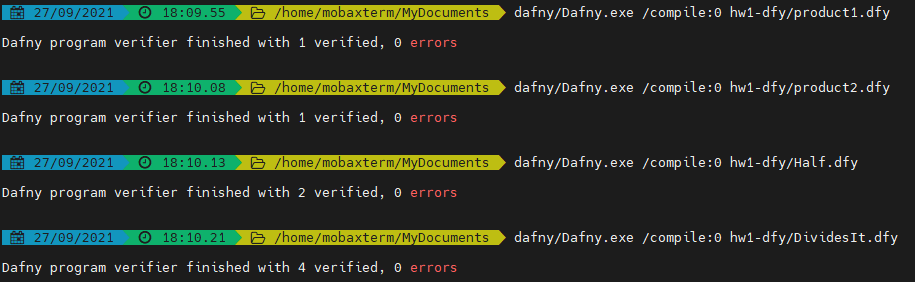
\includegraphics[width=\textwidth]{hw1-dafny-output.png}

\pagebreak

\section*{Problem 2}

\begin{verbatim}
int pm(int x, int y)
@requires x >= 0 & y >= 0;
@ensures res = x * y
{
    a := x;
    b := y;
    res := 0;
    while (a > 0) {
        if ((a mod 2) = 1) then res := res + b;
        a := a div 2;
        @assert a >= 0;
        b := b * 2;
    }
    return res;
}
\end{verbatim}

\paragraph{Loop Invariant} \verb|a>=0 & a*b + res == x*y|

\subsection*{Basic Blocks/Basic Paths}
\subsubsection*{BB1:}
\begin{verbatim}
@requires x >= 0 & y >= 0;
a := x;
b := y;
res := 0;
@invariant a>=0 & a*b + res = x*y;
\end{verbatim}
\textbf{VC1:}
\verb|(x>=0 & y>=0 & a=x & b=y & res=0) ==> (a>=0 & a*b+res=x*y)| for all x, y, a, b, and res.

\subsubsection*{BB2:}
\begin{verbatim}
@invariant a>=0 & a*b + res = x*y;
@assume a > 0;  // while entry condition
@assume ((a mod 2) = 1);  // then-branch
res := res + b;
a := a div 2;
@assert a >= 0;
\end{verbatim}
\textbf{VC2:}\\
\verb|(a0>=0 & a0*b+res0=x*y & a0>0 & ((a0 mod 2)=1) & res1=res0+b & a1=(a0 div 2)) ==> a1>=0| for all x, y, a0, a1, b, res0, res1.

\subsubsection*{BB3:}
\begin{verbatim}
@invariant a>=0 & a*b + res = x*y;
@assume a > 0;  // while entry condition
@assume !((a mod 2) = 1);  // else-branch
a := a div 2;
@assert a >= 0;
\end{verbatim}
\textbf{VC3:}\\
\verb|(a0>=0 & a0*b+res=x*y & a0>0 & !((a0 mod 2)=1) & a1=(a0 div 2)) ==> a1>=0| for all x, y, a0, a1, b, res.

\subsubsection*{BB4:}
\begin{verbatim}
@invariant a>=0 & a*b + res = x*y;
@assume a > 0;  // while entry condition
@assume ((a mod 2) = 1);  // then-branch
res := res + b;
a := a div 2;
b := b * 2;
@invariant a>=0 & a*b + res = x*y
\end{verbatim}
\textbf{VC4:}
\begin{verbatim}
(a0>=0 & a0*b0+res0=x*y & a0>0 & ((a0 mod 2)=1) 
       & res1=res0+b & a1=(a0 div 2) & b1=b0*2) ==> a1*b1+res1=x*y
\end{verbatim}
for all x, y, a0, a1, b0, b1, res0, res1.

\subsubsection*{BB5:}
\begin{verbatim}
@invariant a>=0 & a*b + res = x*y;
@assume a > 0;  // while entry condition
@assume !((a mod 2) = 1);  // else-branch
a := a div 2;
b := b * 2;
@invariant a>=0 & a*b + res = x*y
\end{verbatim}
\textbf{VC5:}
\begin{verbatim}
(a0>=0 & a0*b0+res=x*y & a0>0 & !((a0 mod 2)=1) 
       & a1=(a0 div 2)) & b1=b0*2) ==> a1*b1+res=x*y
\end{verbatim}
for all x, y, a0, a1, b0, b1, res.

\subsubsection*{BB6:}
\begin{verbatim}
@invariant a>=0 & a*b + res = x*y
@assume !(a > 0);  // while exit condition
return res;
@ensures res = x * y;
\end{verbatim}
\textbf{VC6:}
\verb|(a>=0 & a*b+res=x*y & !(a>0)) ==> res=x*y| for all x, y, a, b, res.

\subsection*{SMT Formula}
To check if the verification conditions are valid, each VC is negated and check for UNSAT.
For simplicity, the six negated VCs are combined with a disjunction as below.
If any of negated VCs is satisfiable, the program is not proven correct using the invariant.
Z3 returns UNSAT for the combined SMT formula; hence the program is correct.

\pagebreak

\scriptsize
\begin{verbatim}
; Variable declarations
(declare-fun x () Int)
(declare-fun y () Int)
(declare-fun a () Int)
(declare-fun a0 () Int)
(declare-fun a1 () Int)
(declare-fun b () Int)
(declare-fun b0 () Int)
(declare-fun b1 () Int)
(declare-fun res () Int)
(declare-fun res0 () Int)
(declare-fun res1 () Int)

; Constraints
(assert (or
    ; VC1
    (and (>= x 0) (>= y 0) (= a x) (= b y) (= res 0)
         (not (and (>= a 0) (= (+ (* a b) res) (* x y)))))
    ; VC2
    (and (>= a0 0) (= (+ (* a0 b) res0) (* x y)) (> a0 0) (= (mod a0 2) 1) (= res1 (+ res0 b)) (= a1 (div a0 2))
         (not (>= a1 0)))
    ; VC3
    (and (>= a0 0) (= (+ (* a0 b) res0) (* x y)) (> a0 0) (not (= (mod a0 2) 1)) (= a1 (div a0 2))
         (not (>= a1 0)))
    ; VC4
    (and (>= a0 0) (= (+ (* a0 b0) res0) (* x y)) (> a0 0) (= (mod a0 2) 1) (= res1 (+ res0 b0)) (= a1 (div a0 2)) (= b1 (* b0 2))
         (not (= (+ (* a1 b1) res1) (* x y))))
    ; VC5
    (and (>= a0 0) (= (+ (* a0 b0) res) (* x y)) (> a0 0) (not (= (mod a0 2) 1)) (= a1 (div a0 2)) (= b1 (* b0 2))
         (not (= (+ (* a1 b1) res) (* x y))))
    ; VC6
    (and (>= a 0) (= (+ (* a b) res) (* x y)) (not (> a 0))
         (not (= res (* x y))))
))
(check-sat)
\end{verbatim}

\end{document}